%8 to 20 pages around 50 to 70 ref
%More than a literature review
%Organize related work - impose structure
%Be clear as to how previous work being described relates to your own.
%The reader should not be left wondering why you've described something!!
%Critique the existing work - Where is it strong where is it weak? What are the unreasonable/undesirable assumptions?
%Identify opportunities for more research (i.e., your thesis) Are there unaddressed, or more important related topics?
%After reading this chapter, one should understand the motivation for and importance of your thesis
%You should clearly and precisely define all of the key concepts dealt with in the rest of the thesis, and teach the 
%reader what s/he needs to know to understand the rest of the thesis.

%%% 1 page: overview of what is going on

Using emotional responses to increase the level of users interaction with a real-time 
play technology requires an effective technique to identifying specific emotion 
states within an emotional space. Major existing emotion models in the
psychology literture includes: basic emotion theory ~\cite{ekman1992argument, ekman1992there} ,
dimensional emotion theory ~\cite{lang1995emotion, russell1980circumplex} and models 
from appraisal theory (e.g.,~\cite{roseman2001model}) ~\cite{zhang2010service}

Basic emotion theory identifes anger, disgust, fear, happiness, sadness, and 
surprise ~\cite{peter2006emotion} as the consice set of primary
emotions. These are actually the least six universal categories researchers agreed 
upon ~\cite{zagalo2004story}. It also claims these
primary emotions are distinguishable from each other and
other affective phenomena ~\cite{dalgleish1999handbook}. On the other hand dimensional 
emotion theory argues that all emotional states reside
in a two-dimensional space, defined by arousal and valence.

While there are various opinions on identifying emotional
states, classifcation into discrete emotions ~\cite{dalgleish1999handbook}, or locating
emotions along multiple axes ~\cite{russell1989affect, lang1995emotion}, both 
had limited success in using physiology to identify 
emotional states ~\cite{cacioppo2000psychophysiology}.

Lang used a 2-D space defined by arousal and valence (pleasure) (AV space) 
to classify emotions ~\cite{lang1995emotion}. Valence can be
described as a subjective feeling of pleasantness or unpleasantness while 
arousal is the subjective state feeling activated
or deactivated ~\cite{barrett1998discrete}. Using an arousal-valence space to create
the Affect Grid, Russell believed that arousal and valence
are cognitive dimentions of individual emotion states. Affect is a broad definition 
that includes feelings, moods, sentiments etc. and is commonly used to define the concept of
emotion ~\cite{picard2003affective}. Russell's circumplex model has two "axes"
that might be labeled as displeasure/pleasure (horizontal
axis) and low/high arousal (vertical axis) It is not easy to
map affective states into distinctive emotional states, However these models can 
provide a mapping between predefined
states and the level of arousal and valence ~\cite{zagalo2004story}, 
Figure ~\ref{fig:russelavspace}.

\begin{figure}[h!]
  \caption[Russell's arousal and valence model]
  {Russell's circumplex model with two axes of arousal and valence \footnotemark.}
  \centering
  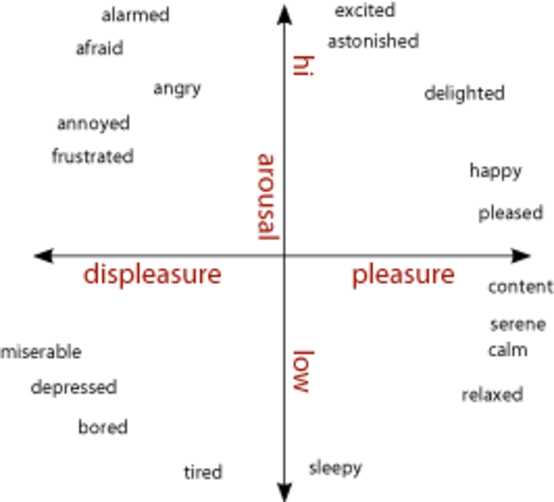
\includegraphics[width=0.5\textwidth]{images/russell-av-space.pdf}
  \label{fig:russelavspace}
\end{figure}

\footnotetext{Photo credit: http://imagine-it.org/gamessurvey/}

Both mentioned models for identifying emotions convey some
practical issues in emotion measurement. In a HCI context, the 
stimuli for potential emotions may vary less than
in human-human interaction (e.g., participant verbal expressions and body language) 
~\cite{zhang2010service} and also the combination of
evoked emotions ~\cite{peter2006emotion}. However with help of physiological
signals and the fuzzy logic in the model we are going to
use, such issues with our dimentional emotion models would
be minimized. Though it is anticipated to observe different range 
of evoked emotions while interacting with play
technologies compared to interacting with other humans in
daily life. ~\cite{zhang2010service}. However our dimensional emotion models
suffers some other problems. One problems is that arousal
and valence are not independent and one can impact the
other ~\cite{mandryk2007fuzzy}. Continuously capturing emotional experiences
in this applied setting is of its other halmarks. Subjective
measures based on dimensional emotion theory, such as the
Affect Grid ~\cite{russell1989affect} and the Self-Assessment 
Manikin ~\cite{bradley1994measuring}, allow
for quick assessments of user emotional experiences but they
may aggregate responses over the course of many events ~\cite{zhang2010service}.
This work uses Mandryk et al. version of AV space ~\cite{mandryk2007fuzzy}.


\section{Why Do We Play?}
%%% 3 pages: what are games for and why do we play them
%%% the importance of being challenged for people, and how it helps them to develop

lazzaro2004we---
others enjoy the challenge and chance to test their abilities. Games offer an efficiency 
and order in playing that they want in life. They value the sensations from doing new 
things such as dirt-bike racing or flying, that they otherwise lack the skills, 
resources, or social permission to do. A few like to escape the real world; others 
enjoy escaping its social norms. Nearly all enjoy the feeling of challenge and complete 
absorption. The exciting and relaxing effects of games is very appealing and some apply 
its therapeutic benefits to "get perspective," calm down after a hard day, or build 
self-esteem. Direct observation reveals details about player emotion. We find emotion 
in player's visceral, behavioral, cognitive, and social responses to games. Players play 
to experience these body sensations that result from and drive their actions. Some crave 
the increased heart rate of excitement from a race, the skin prickling sensation from 
Wonder, or the tension of Frustration followed by feelings of Fiero. For others it is 
simply the exchange of worries and thought and feelings for relaxation and contentment 
or a feeling of achievement knowing they did it right. ---lazzaro2004we

Playing video games as a kind of entertainment would help people to have new internal 
experiences. The virtual world of video games let adults to play as new rolls and enjoy filling 
their heads with new throughts and emotions. Some people value 
the sensation

Games are opportunities for development and design of environemnts therefore 
the player can interactively experience various emotions and mental conditions.
This interactive experience in contrast to movies 
and other major types of digital entertainment is what makes them exceptional

\section{Play Technologies and Human Body}
%%% 5 pages: human body and play technologies
%%% getting challenged and physiological signals, the importance of GSR

\section{Adaptive Play Technologies}
%%% 10 pages: adaptive play technologies critique existing systems (easy medium hard system), ideas
%%% , problems and challenges, works has been done, goals for this study and future works.
%%% adapting play technologies by chaning Player, NPC, Environment parameters.
